\chapter{Espacio de Wiener y caos}

\section{Proceso isonormal}
La familia $\{W(h):h\in\Hil\}$ es un proceso gaussiano centrado con
$\E[W(h)W(g)]=\ip{h}{g}$. Denotamos por $He_n$ los polinomios de Hermite
probabilistas,
\[
  He_n(x) = (-1)^n e^{x^2/2}\frac{\dd^n}{\dd x^n}e^{-x^2/2},\qquad
  e^{tx-t^2/2}=\sum_{n\ge0}\frac{t^n}{n!}He_n(x).
\]

\section{Descomposición en caos}
\begin{teorema}[Wiener--Itô]
Toda $F\in L^2(\Omega,\F_T,\Prob)$ admite el desarrollo ortogonal
\[
  F = \sum_{n=0}^\infty I_n(f_n),\qquad \E[F^2]=\sum_{n\ge0} n!\,\norm{f_n}^2_{L^2([0,T]^n)},
\]
con $f_n$ simétricas y $I_n$ la integral múltiple de Itô.
\end{teorema}

Para funcionales que sólo dependen de $W_T$ basta con $h=\ind_{[0,T]}$:
$I_n(\ind_{[0,T]}^{\otimes n}) = T^{n/2} He_n(W_T/\sqrt T)$. Si $F=f(W_T)$ y $Z=W_T/\sqrt T$,
\[
  F=\sum_{n\ge0} a_n He_n(Z),\qquad a_n=\frac{\E[f(\sqrt T Z)He_n(Z)]}{n!},\qquad
  \operatorname{Var}(F)=\sum_{n\ge1} n!\,a_n^2.
\]

\begin{ejemplo}[Martingala exponencial]
$\exp(\sigma W_T-\tfrac12\sigma^2T)=\sum_n \frac{(\sigma\sqrt T)^n}{n!}He_n(Z)$:
el precio descontado de un activo log-normal vive en todos los caos con pesos
que decaen factorialmente.
\end{ejemplo}

\begin{figure}[h]
  \centering
  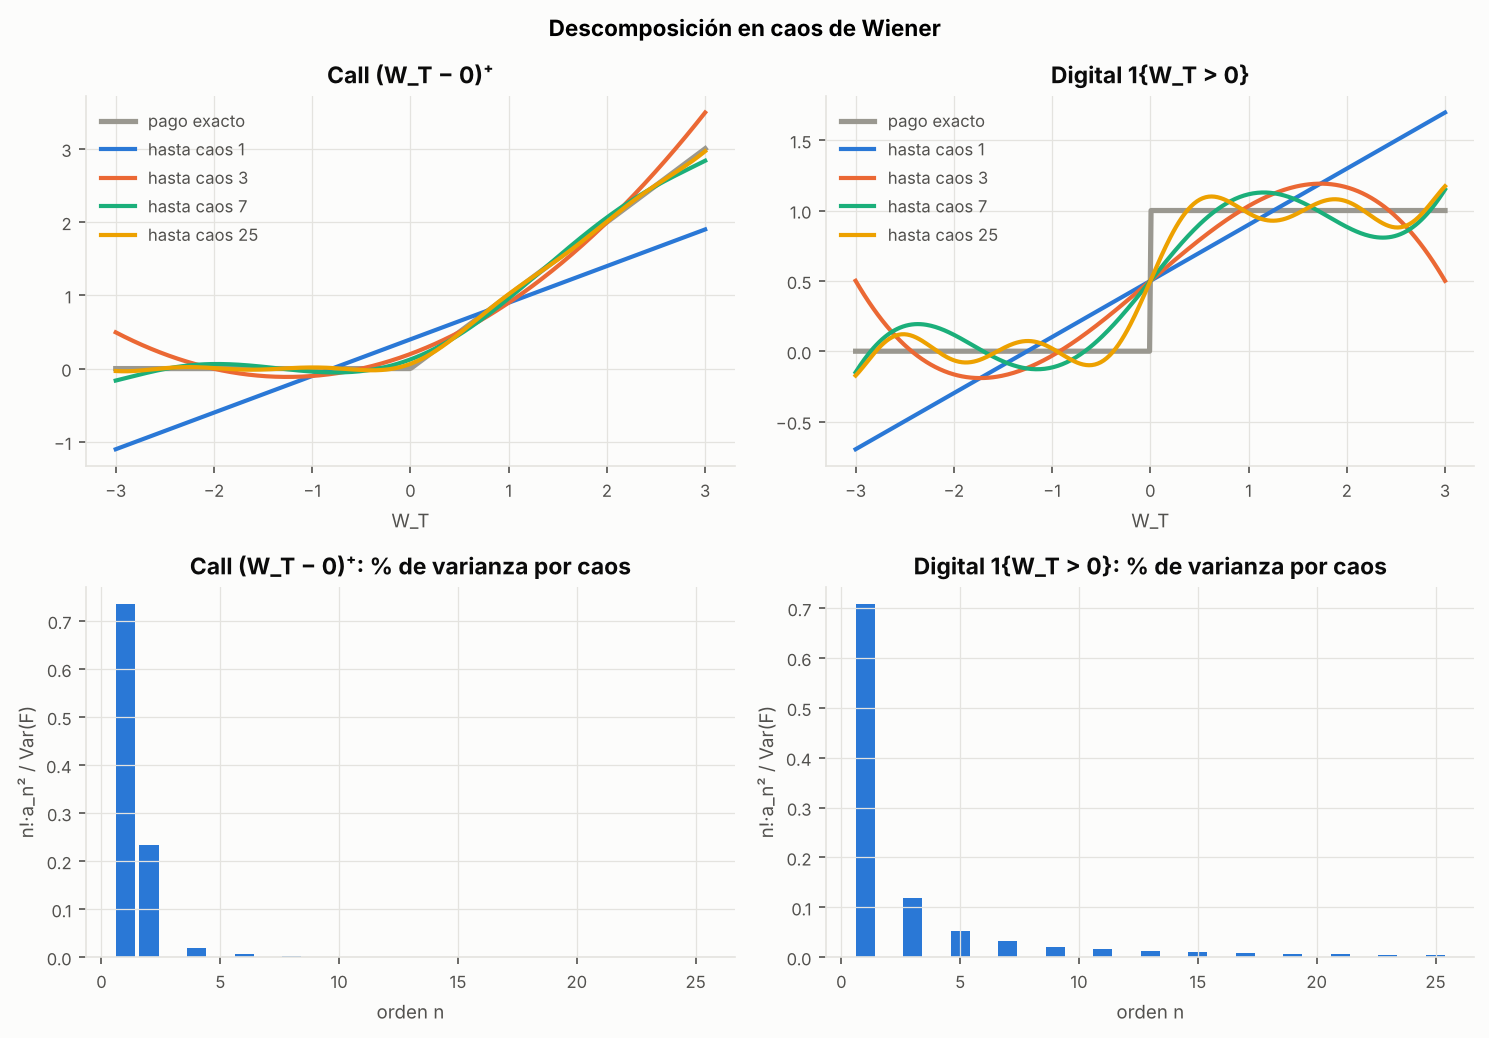
\includegraphics[width=\linewidth]{01_caos_de_wiener}
  \caption{Truncaciones del desarrollo en caos y energía por orden para una call
  y una digital (\codigo{examples/01\_caos\_de\_wiener.py}). La discontinuidad de la
  digital reparte la varianza en caos altos: decaimiento lento $\Rightarrow$ menor
  regularidad Malliavin.}
\end{figure}
